\documentclass[10pt,letterpaper,english,hidelinks]{amsart}

\usepackage{amsmath}
\usepackage{amssymb}
\usepackage{amsthm}
\usepackage{fancyhdr}
\usepackage{graphicx}
\usepackage{pgfplots}
\usepackage{tikz}
\usepackage{datetime2}
\usepackage{natbib}
\usepackage[unicode]{hyperref}
\usepackage{mathtools}
\mathtoolsset{showonlyrefs}

\usetikzlibrary{fadings}
\usetikzlibrary{patterns}
\usetikzlibrary{shadows.blur}
\usetikzlibrary{arrows}
\usetikzlibrary{decorations.markings}
\usetikzlibrary{positioning}
\usetikzlibrary{calc}
\usetikzlibrary{math}

\pgfplotsset{compat=1.16}

\DTMnewdatestyle{mydateformat}{%
  \renewcommand{\DTMdisplaydate}[4]{%
    \number##1\ % year
    \DTMenglishmonthname{##2}\ % Month
    \number##3% day
  }%
  \renewcommand{\DTMDisplaydate}{\DTMdisplaydate}%
}
\DTMsetdatestyle{mydateformat}

% text dimensions
\setlength{\textwidth}{6.5in}
\setlength{\textheight}{9in}

% adjust top margins
\setlength{\topmargin}{0in}
\setlength{\voffset}{-30pt}
\setlength{\headheight}{12pt}

% no room for notes on the side
\setlength{\oddsidemargin}{0in}
\setlength{\evensidemargin}{0in}
\setlength{\marginparwidth}{0in}

% space between paragraphs and lines
\setlength{\parskip}{5pt}
\linespread{1.05} % for final submission
% \linespread{2} % for editing drafts

% Hyphenation
\numberwithin{equation}{section}
\hyphenation{semi-stable}

% Numbering for Theorems, Lemmas, etc.
\theoremstyle{plain}
\newtheorem{theorem}{Theorem}[section]
\newtheorem{corollary}[theorem]{Corollary}
\newtheorem{lemma}[theorem]{Lemma}
\newtheorem{conjecture}[theorem]{Conjecture}
\theoremstyle{definition}
\newtheorem{definition}[theorem]{Definition}
\newtheorem{example}[theorem]{Example}
\newtheorem{remark}[theorem]{Remark}
\numberwithin{equation}{section}

% Header Definitions
\fancyhead[L]{\nouppercase{\rightmark}}
\fancyhead[R]{\nouppercase{\leftmark}}

\pagestyle{fancy}

\newcommand{\cech}{\v{C}ech }
\DeclareMathOperator{\Cech}{\textrm{\v{C}ech}}
\DeclareMathOperator{\Ima}{Im}
\DeclareMathOperator{\Ker}{Ker}
\DeclareMathOperator{\nul}{Null}
\DeclareMathOperator{\boundary}{\partial}
\newcommand*{\Z}{\mathbb{Z}}
\newcommand{\bigslant}[2]{%
  \mathchoice
  {{\raisebox{.2em}{$#1$}\left/\raisebox{-.2em}{$#2$}\right.}}
  {{\raisebox{0em}{$#1$}\left/\raisebox{0em}{$#2$}\right.}}
  {{\raisebox{0em}{$#1$}\left/\raisebox{0em}{$#2$}\right.}}
  {{\raisebox{0em}{$#1$}\left/\raisebox{0em}{$#2$}\right.}}
}
\newcommand{\cross}{\times}
\newcommand{\normalsubgroup}{\triangleleft}
\newcommand{\figref}[1]{[Fig. \ref{#1}]}
\newcommand{\subfigref}[2]{[Fig. \ref{#1}, #2]}
\newcommand{\red}[1]{{\color{red} #1}}
\newcommand{\lightgray}[1]{{\color{lightgray} #1}}


\title[Persistent Homology]{Persistent Homology: Computations and Applications}
\author{Stephen Ermshar}
\address{Department of Mathematics, Walla Walla University, College Place, WA 99324}
\date{\DTMDisplaydate{2020}{5}{29}{}} % pre-final draft due
\thanks{Advisor: Dr. John Foster}

% for keeping track of printed drafts, adds date and time to every page
\thanks{\tiny{\DTMtoday, \DTMcurrenttime}}
\rfoot{\hfill\newline\tiny{\DTMtoday, \DTMcurrenttime}}


\begin{document}

\begin{abstract}
    % 300 word abstract.
    Persistent Homology is a method for understanding a numerical multi dimensional data set by observing certain features of shapes generated by the data.
    These features of interest are holes, and can provide clues for how the data is connected or where data may be missing.
    Homology is the study of these holes, and Persistent Homology is a natural application of this topic to data sets.
    This paper will provide an introduction to Simplicial Homology and how it can be applied to a data set.
\end{abstract}
\maketitle

\section{Introduction}


Persistent homology is a tool for understanding the shape of a data set.
If a data set is a collection of points in two dimensional space, then it can be graphed in a plane.
We can easily look at the graph and see whether the data clumps together in certain places, or if it forms more interesting shapes, like loops.
We can graph data from one and three dimensions as well, but with dimensions four and higher we are no longer able to visualize the data in a traditional scatter plot.

\begin{figure}[h]
    \centering
    \scalebox{0.75}{\tikzset{
pattern size/.store in=\mcSize,
pattern size = 5pt,
pattern thickness/.store in=\mcThickness,
pattern thickness = 0.3pt,
pattern radius/.store in=\mcRadius,
pattern radius = 1pt}
\makeatletter
\pgfutil@ifundefined{pgf@pattern@name@_iy1rqtf17}{
\pgfdeclarepatternformonly[\mcThickness,\mcSize]{_iy1rqtf17}
{\pgfqpoint{0pt}{0pt}}
{\pgfpoint{\mcSize+\mcThickness}{\mcSize+\mcThickness}}
{\pgfpoint{\mcSize}{\mcSize}}
{
\pgfsetcolor{\tikz@pattern@color}
\pgfsetlinewidth{\mcThickness}
\pgfpathmoveto{\pgfqpoint{0pt}{0pt}}
\pgfpathlineto{\pgfpoint{\mcSize+\mcThickness}{\mcSize+\mcThickness}}
\pgfusepath{stroke}
}}
\makeatother

% https://ipfs-sec.stackexchange.cloudflare-ipfs.com/tex/A/question/6135.html
\tikzset{every picture/.style={line width=0.75pt, opacity=0}} %set default line width to 0.75pt
\tikzset{onslide/.code args={<#1>#2}{%
    \only<#1>{\pgfkeysalso{#2}} % \pgfkeysalso doesn't change the path
}}

\begin{tikzpicture}[x=0.75pt,y=0.75pt,yscale=-1,xscale=1]

    \def\points{
        (240,312),
        (230,238),
        (282,164),
        (300,320),
        (348,180),
        (348,336),
        (398,262),
        (406,322)
    }

    % \def\points{
    %     (134,150),
    %     (166,136),
    %     (118,298),
    %     (178,312),
    %     (114,222),
    %     (232,342),
    %     (322,232),
    %     (316,324),
    %     (280,342),
    %     (504,284),
    %     (418,350),
    %     (388,184),
    %     (292,126),
    %     (324,172),
    %     (234,108),
    %     (246,154),
    %     (162,192),
    %     (458,210),
    %     (362,348)
    % }

    \foreach \r [count=\ri from 2] in {40, 50, 60, 85}{
        \foreach \p in \points{
            \draw
                [color={rgb, 255:red, 165; green, 232; blue, 255}]
                [fill={rgb, 255:red, 165; green, 232; blue, 255}]
                [onslide=<{\ri}>{opacity=1}]
                [line width=0]
                \p circle
                [radius=\r];
        }
        \foreach \a [count=\ai] in \points{
            \foreach \b [count=\bi] in \points{
                \path \a;
                \pgfgetlastxy{\ax}{\ay}
                \path \b;
                \pgfgetlastxy{\bx}{\by}
                \pgfmathsetmacro\thresh{2*\r}
                % The 23 on the following line is there because
                % this calculation connected some vertices before the
                % circles drawn underneath overlapped. the adjustment
                % doesn't appear to make the graph incorrect and forces
                % the vertices to wait longer before connecting, though
                % it is concerning.
                \pgfmathsetmacro\dist{veclen(\ax-\bx,\ay-\by)+23}
                \ifnum\ai<\bi
                    \ifdim\dist pt<\thresh pt
                        \draw
                        [onslide=<{\ri}>{opacity=1}]
                        \a -- \b;
                    \fi
                \fi

            }
        }
    }

    % Vertices go at the bottom so they're on top of the rest
    \foreach \p [count=\pi] in \points{
        \draw
            [black, fill=black]
            [opacity=1]
            \p circle
            [radius= 3.35];
        % \draw % mark nodes for debugging
        %     [opacity=1]
        %     \x+(10,10) node {\(\pi\)};
    }

\end{tikzpicture}
}
    \caption{}
    \label{fig:persistence-demo-r25}
\end{figure}

To get an idea of the shape formed by a data set we connect nearby points, using a threshold radius to determine whether points are close enough to be considered related.
With the resulting graph-like structure we can apply tools from homology to find holes like the two shown in figure \ref{fig:persistence-demo-r25}.
Homology will help us find higher dimensional analogues of these holes as well, such as voids, which are the space inside an enclosed surface.

The graph-like structure, which is called a simplicial complex, will change depending on the value of the radius.
If the radius is small enough then no points will be connected, and if it is large enough then all the points will be connected.
As the radius varies between these two extremes more interesting simplicial complexes result.
If the radius is increased holes will form as points begin to connect, and eventually as more points connect those holes will get filled in.
The holes that persist over a wide range of radius values are considered to be the more significant features of the shape.

In section \ref{sec:homology} we'll formalize the simplicial complex and its building blocks.
Then, given an existing simplicial complex we'll solidify the concept with an example computation for finding a hole.
As we move on to persistent homology in section \ref{sec:persistent-homology} we'll introduce the cech complex, which is used to build a simplicial complex given a data set and a radius.
Having calculated the homology for the cech complex along a range of scales we'll look at two methods for visualizing the results, and \red{might} look at the stability theorem, which will ensure that the results are reliable.
Finally, in section \ref{sec:applications} we \red{might} explore applications for persistent homology.

\section{Homology}\label{sec:homology}

\subsection{Simplicial Homology}\label{sec:simplicial-homology}

The basic building block of a simplicial complex is an \(n\)-simplex.
An \(n\)-simplex generalizes the triangle to \(n\) dimensions by associating \(n+1\) vertices with each other in an ordered tuple.
For instance, a point is a 0-simplex, an edge a 1-simplex, a triangle a 2-simplex, a tetrahedron a 3-simplex, and so on \figref{fig:basic-simplices}.

\begin{figure}
    \tikzset{every picture/.style={line width=0.75pt}} %set default line width to 0.75pt

\begin{tikzpicture}[x=0.75pt,y=0.75pt,yscale=-1,xscale=1]

\coordinate (01) at (77,72);
\coordinate (11) at (147,71);
\coordinate (12) at (179,59.5);
\coordinate (21) at (233.21,91.12);
\coordinate (22) at (276.15,74.49);
\coordinate (23) at (239.92,44.11);
\coordinate (31) at (320,65.5);
\coordinate (32) at (345,30.5);
\coordinate (33) at (369,65.5);
\coordinate (34) at (342,90.5);

% 0 Simplex
\draw   [black, fill=black] (01) circle [radius= 3.35] ;

% 1 Simplex
\draw   [black, fill=black] (11) circle [radius= 3.35] ;
\draw   [black, fill=black] (12) circle [radius= 3.35] ;
\draw   (11) -- (12) ;

% 2 Simplex
\draw   [black, fill=lightgray] (21) -- (22) -- (23) -- cycle   ;
\draw   [black, fill=black] (21) circle [radius= 3.35] ;
\draw   [black, fill=black] (22) circle [radius= 3.35] ;
\draw   [black, fill=black] (23) circle [radius= 3.35] ;

% 3 Simplex
\draw   [black, fill=lightgray] (31) -- (32) -- (34) -- cycle   ;
\draw   [black, fill=gray]      (32) -- (33) -- (34) -- cycle   ;
\draw   [dash pattern={on 4.5pt off 4.5pt}]  (31) -- (33) ;
\draw   [black, fill=black] (31) circle [radius= 3.35] ;
\draw   [black, fill=black] (32) circle [radius= 3.35] ;
\draw   [black, fill=black] (33) circle [radius= 3.35] ;
\draw   [black, fill=black] (34) circle [radius= 3.35] ;

% Straight Arrow
\draw [shift={(163,65.25)}, rotate = 520.23] [fill={rgb, 255:red, 0; green, 0; blue, 0 }  ][line width=0.08]  [draw opacity=0] (8.93,-4.29) -- (0,0) -- (8.93,4.29) -- cycle    ;

% Circle Arrow
\draw  [draw opacity=0] (255.97,69.08) .. controls (255.99,69.3) and (256,69.52) .. (256,69.75) .. controls (256,73.48) and (252.87,76.5) .. (249,76.5) .. controls (245.13,76.5) and (242,73.48) .. (242,69.75) .. controls (242,66.02) and (245.13,63) .. (249,63) .. controls (249.81,63) and (250.59,63.13) .. (251.32,63.38) -- (249,69.75) -- cycle ; \draw   (255.97,69.08) .. controls (255.99,69.3) and (256,69.52) .. (256,69.75) .. controls (256,73.48) and (252.87,76.5) .. (249,76.5) .. controls (245.13,76.5) and (242,73.48) .. (242,69.75) .. controls (242,66.02) and (245.13,63) .. (249,63) .. controls (249.81,63) and (250.59,63.13) .. (251.32,63.38) ;
\draw  [fill={rgb, 255:red, 0; green, 0; blue, 0 }  ,fill opacity=1 ] (253.25,70.52) -- (255.25,65.85) -- (258.47,69.77) ;


% Caption Labels
\draw (78,116)   node   [align=left] {0-simplex};
\draw (166,117)  node   [align=left] {1-simplex};
\draw (256,117)  node   [align=left] {2-simplex};
\draw (347,116)  node   [align=left] {3-simplex};
\draw (78,136)   node   [align=left] {(1)};
\draw (166,137)  node   [align=left] {(1,2)};
\draw (256,137)  node   [align=left] {(1,2,3)};
\draw (347,136)  node   [align=left] {(1,2,3,4)};

% Vertex Labels
\draw (01)+(-10,5)  node   [align=left] {1};
\draw (11)+(-10,5)  node   [align=left] {1};
\draw (12)+(10,5)   node   [align=left] {2};
\draw (21)+(-10,5)  node   [align=left] {1};
\draw (22)+(10,5)   node   [align=left] {2};
\draw (23)+(-10,5)  node   [align=left] {3};
\draw (31)+(-10,5)  node   [align=left] {1};
\draw (32)+(10,0)   node   [align=left] {2};
\draw (33)+(10,5)   node   [align=left] {3};
\draw (34)+(-10,5)  node   [align=left] {4};




\end{tikzpicture}

    \caption{}
    \label{fig:basic-simplices}
\end{figure}

A simplicial complex will be a collection of simplices.
For a simplex to be considered part of a simplicial complex it will need to have been built up from lower dimensional simplices.
A triangle includes its three edges and three vertices, so if a triangle is included in a simplicial complex we will require that all of its edges and vertices are also included in the complex.

\begin{definition}\label{def:simplicial-complex}
    A \textbf{Simplicial Complex} is a finite collection of finite sets such that every subset of every element in the collection is also an element in the collection. \cite{wagner}
\end{definition}

This will be a useful property because when we study the homology of the complex we will be comparing the boundaries of its \(n\)-simplices, which are \((n-1)\)-simplices, to other \((n-1)\)-simplices in the complex.

In general, homology will be calculated by finding all the \((n-1)\)-simplices that form loops, and factoring out any \((n-1)\)-simplices that form loops around \(n\)-simplices, leaving only loops of \((n-1)\)-simplices that surround empty space that could be filled with \(n\)-simplices. These remaining loops are what we intuitively call holes.

% this paragraph is partially redundant
This will allow us to describe holes easily.
An \(n\)-dimensional hole can be thought of as a space surrounded by \(n\)-simplices.
The loops from figure \ref{fig:persistence-demo-r25} are one dimensional holes; the empty space inside a closed surface, like the inside of a hollow tetrahedron, is a two-dimensional hole; the space between separate components of the complex is a zero dimensional hole.
The description of a zero dimensional hole is somewhat different from the others.
When we calculate the homology for a zero dimensional hole we will see the number of connected components, rather than the number of pairs of separate components between which there is empty space.

% this paragraph needs to be reworded, and is redundant
To keep track of signs later on, we'll give each simplex an orientation which will be denoted by the order in which its points are listed.
We'll arbitrarily choose to list the points in increasing order of the point's label.
The resulting simplicial complex will be a graph-like structure, where pairs of connected points are connected by a line, triples by a triangle, four points by a tetrahedron, and \(n\) points by the \(n\)-dimensional analog of a triangle.

% this paragraph needs to be removed, reworded, or moved to the persistence sec.
The radius \(r\) used in the \v{C}ech Complex is the scale parameter that we'll vary when looking for persistence. One can observe that the \v{C}ech Complex fits the definition of a simplicial complex.
Since if the balls around some points intersect, then the balls around any subset of those points must also intersect.

% this paragraph needs to be moved to persistence sec. but the \(C\) part stays
In figure \ref{fig:example-cech} we start with the points labeled \(1\), \(2\), \(3\), and \(4\). We choose a value for \(r\) and construct a cech complex \(C = \{ (1,2,3), (1,2), (1,3), (2,3), (2,4), (3,4), (1), (2), (3), (4) \}\). With this complex we can fill in the remaining triangle and edges in the graph based on the simplices included in the complex. We can visually observe that this complex has one hole surrounded by \(1\)-simplices \((2,3)\), \((3,4)\), and \((2,4)\).

\subsection{Computations}

\begin{figure}
    \centering
    \begin{minipage}{.5\textwidth}
        \centering
        \tikzset{
pattern size/.store in=\mcSize,
pattern size = 5pt,
pattern thickness/.store in=\mcThickness,
pattern thickness = 0.3pt,
pattern radius/.store in=\mcRadius,
pattern radius = 1pt}
\makeatletter
\pgfutil@ifundefined{pgf@pattern@name@_iy1rqtf17}{
\pgfdeclarepatternformonly[\mcThickness,\mcSize]{_iy1rqtf17}
{\pgfqpoint{0pt}{0pt}}
{\pgfpoint{\mcSize+\mcThickness}{\mcSize+\mcThickness}}
{\pgfpoint{\mcSize}{\mcSize}}
{
\pgfsetcolor{\tikz@pattern@color}
\pgfsetlinewidth{\mcThickness}
\pgfpathmoveto{\pgfqpoint{0pt}{0pt}}
\pgfpathlineto{\pgfpoint{\mcSize+\mcThickness}{\mcSize+\mcThickness}}
\pgfusepath{stroke}
}}
\makeatother
\tikzset{every picture/.style={line width=0.75pt}} %set default line width to 0.75pt

\begin{tikzpicture}[x=0.75pt,y=0.75pt,yscale=-1,xscale=1]
%uncomment if require: \path (0,95); %set diagram left start at 0, and has height of 95

\draw [shift={(163,23.5)}, rotate = 99.21] [color={rgb, 255:red, 165; green, 232; blue, 255}  ][fill={rgb, 255:red, 165; green, 232; blue, 255 }  ][line width=0]      (0, 0) circle [x radius= 20, y radius= 20]   ;
\draw [shift={(135,40)}, rotate = 349.29] [color={rgb, 255:red, 165; green, 232; blue, 255}  ][fill={rgb, 255:red, 165; green, 232; blue, 255 }  ][line width=0]      (0, 0) circle [x radius= 20, y radius= 20]   ;
\draw [shift={(13,61)}, rotate = 312.63] [color={rgb, 255:red, 165; green, 232; blue, 255}  ][fill={rgb, 255:red, 165; green, 232; blue, 255 }  ][line width=0]      (0, 0) circle [x radius= 20, y radius= 20]   ;
\draw [shift={(56,17)}, rotate = 0] [color={rgb, 255:red, 165; green, 232; blue, 255}  ][fill={rgb, 255:red, 165; green, 232; blue, 255 }  ][line width=0]      (0, 0) circle [x radius= 20, y radius= 20]   ;
\draw [shift={(69,54)}, rotate = 329.74] [color={rgb, 255:red, 165; green, 232; blue, 255}  ][fill={rgb, 255:red, 165; green, 232; blue, 255 }  ][line width=0]      (0, 0) circle [x radius= 20, y radius= 20]   ;
\draw [shift={(95,25)}, rotate = 353.99] [color={rgb, 255:red, 165; green, 232; blue, 255}  ][fill={rgb, 255:red, 165; green, 232; blue, 255 }  ][line width=0]      (0, 0) circle [x radius= 20, y radius= 20]   ;
\draw [shift={(95,25)}, rotate = 69.78] [color={rgb, 255:red, 165; green, 232; blue, 255}  ][fill={rgb, 255:red, 165; green, 232; blue, 255 }  ][line width=0]      (0, 0) circle [x radius= 20, y radius= 20]   ;
\draw [shift={(135,40)}, rotate = 314.34] [color={rgb, 255:red, 165; green, 232; blue, 255}  ][fill={rgb, 255:red, 165; green, 232; blue, 255 }  ][line width=0]      (0, 0) circle [x radius= 20, y radius= 20]   ;
\draw [shift={(157,60.5)}, rotate = 31.29] [color={rgb, 255:red, 165; green, 232; blue, 255}  ][fill={rgb, 255:red, 165; green, 232; blue, 255 }  ][line width=0]      (0, 0) circle [x radius= 20, y radius= 20]   ;
\draw [shift={(157,60.5)}, rotate = 349.29] [color={rgb, 255:red, 165; green, 232; blue, 255}  ][fill={rgb, 255:red, 165; green, 232; blue, 255 }  ][line width=0]      (0, 0) circle [x radius= 20, y radius= 20]   ;
\draw [shift={(157,60.5)}, rotate = 99.21] [color={rgb, 255:red, 165; green, 232; blue, 255}  ][fill={rgb, 255:red, 165; green, 232; blue, 255 }  ][line width=0]      (0, 0) circle [x radius= 20, y radius= 20]   ;
\draw [shift={(56,17)}, rotate = 312.63] [color={rgb, 255:red, 165; green, 232; blue, 255}  ][fill={rgb, 255:red, 165; green, 232; blue, 255 }  ][line width=0]      (0, 0) circle [x radius= 20, y radius= 20]   ;
\draw [shift={(95,25)}, rotate = 31.29] [color={rgb, 255:red, 165; green, 232; blue, 255}  ][fill={rgb, 255:red, 165; green, 232; blue, 255 }  ][line width=0]      (0, 0) circle [x radius= 20, y radius= 20]   ;
\draw [shift={(95,25)}, rotate = 0] [color={rgb, 255:red, 165; green, 232; blue, 255}  ][fill={rgb, 255:red, 165; green, 232; blue, 255 }  ][line width=0]      (0, 0) circle [x radius= 20, y radius= 20]   ;
\draw [shift={(69,54)}, rotate = 36.87] [color={rgb, 255:red, 165; green, 232; blue, 255}  ][fill={rgb, 255:red, 165; green, 232; blue, 255 }  ][line width=0]      (0, 0) circle [x radius= 20, y radius= 20]   ;
\draw [shift={(56,17)}, rotate = 36.87] [color={rgb, 255:red, 165; green, 232; blue, 255}  ][fill={rgb, 255:red, 165; green, 232; blue, 255 }  ][line width=0]      (0, 0) circle [x radius= 20, y radius= 20]   ;
\draw [shift={(95,25)}, rotate = 329.74] [color={rgb, 255:red, 165; green, 232; blue, 255}  ][fill={rgb, 255:red, 165; green, 232; blue, 255 }  ][line width=0]      (0, 0) circle [x radius= 20, y radius= 20]   ;
\draw [shift={(163,23.5)}, rotate = 353.99] [color={rgb, 255:red, 165; green, 232; blue, 255}  ][fill={rgb, 255:red, 165; green, 232; blue, 255 }  ][line width=0]      (0, 0) circle [x radius= 20, y radius= 20]   ;
\draw [shift={(135,40)}, rotate = 69.78] [color={rgb, 255:red, 165; green, 232; blue, 255}  ][fill={rgb, 255:red, 165; green, 232; blue, 255 }  ][line width=0]      (0, 0) circle [x radius= 20, y radius= 20]   ;
\draw [shift={(163,23.5)}, rotate = 314.34] [color={rgb, 255:red, 165; green, 232; blue, 255}  ][fill={rgb, 255:red, 165; green, 232; blue, 255 }  ][line width=0]      (0, 0) circle [x radius= 20, y radius= 20]   ;
\draw [shift={(255, 50)}, rotate = 314.34] [color={rgb, 255:red, 165; green, 232; blue, 255}  ][fill={rgb, 255:red, 165; green, 232; blue, 255 }  ][line width=0]      (0, 0) circle [x radius= 20, y radius= 20]   ;

%Straight Lines [id:da20686486428426965] (1-2)
% \draw    (13,61) -- (56,17) ;
\draw [shift={(56,17)}, rotate = 312.63] [color={rgb, 255:red, 0; green, 0; blue, 0 }  ][fill={rgb, 255:red, 0; green, 0; blue, 0 }  ][line width=0.75]      (0, 0) circle [x radius= 3.35, y radius= 3.35]   ;
\draw [shift={(13,61)}, rotate = 312.63] [color={rgb, 255:red, 0; green, 0; blue, 0 }  ][fill={rgb, 255:red, 0; green, 0; blue, 0 }  ][line width=0.75]      (0, 0) circle [x radius= 3.35, y radius= 3.35]   ;
%Straight Lines [id:da9899744043809231] (2-4)
\draw    (56,17) -- (95,25) ;
% \draw [shift={(95,25)}, rotate = 0] [color={rgb, 255:red, 0; green, 0; blue, 0 }  ][fill={rgb, 255:red, 0; green, 0; blue, 0 }  ][line width=0.75]      (0, 0) circle [x radius= 3.35, y radius= 3.35]   ;
% \draw [shift={(56,17)}, rotate = 0] [color={rgb, 255:red, 0; green, 0; blue, 0 }  ][fill={rgb, 255:red, 0; green, 0; blue, 0 }  ][line width=0.75]      (0, 0) circle [x radius= 3.35, y radius= 3.35]   ;
%Straight Lines [id:da4483952202454973] (2-3)
\draw    (56,17) -- (69,54) ;
\draw [shift={(69,54)}, rotate = 36.87] [color={rgb, 255:red, 0; green, 0; blue, 0 }  ][fill={rgb, 255:red, 0; green, 0; blue, 0 }  ][line width=0.75]      (0, 0) circle [x radius= 3.35, y radius= 3.35]   ;
\draw [shift={(56,17)}, rotate = 36.87] [color={rgb, 255:red, 0; green, 0; blue, 0 }  ][fill={rgb, 255:red, 0; green, 0; blue, 0 }  ][line width=0.75]      (0, 0) circle [x radius= 3.35, y radius= 3.35]   ;
%Straight Lines [id:da013663715151336797](3-4)
\draw    (69,54) -- (95,25) ;
\draw [shift={(95,25)}, rotate = 329.74] [color={rgb, 255:red, 0; green, 0; blue, 0 }  ][fill={rgb, 255:red, 0; green, 0; blue, 0 }  ][line width=0.75]      (0, 0) circle [x radius= 3.35, y radius= 3.35]   ;
\draw [shift={(69,54)}, rotate = 329.74] [color={rgb, 255:red, 0; green, 0; blue, 0 }  ][fill={rgb, 255:red, 0; green, 0; blue, 0 }  ][line width=0.75]      (0, 0) circle [x radius= 3.35, y radius= 3.35]   ;
%Straight Lines [id:da6445202628566384](4-7)
% \draw    (95,25) -- (163,23.5) ;
\draw [shift={(163,23.5)}, rotate = 353.99] [color={rgb, 255:red, 0; green, 0; blue, 0 }  ][fill={rgb, 255:red, 0; green, 0; blue, 0 }  ][line width=0.75]      (0, 0) circle [x radius= 3.35, y radius= 3.35]   ;
\draw [shift={(95,25)}, rotate = 353.99] [color={rgb, 255:red, 0; green, 0; blue, 0 }  ][fill={rgb, 255:red, 0; green, 0; blue, 0 }  ][line width=0.75]      (0, 0) circle [x radius= 3.35, y radius= 3.35]   ;
%Straight Lines [id:da3743946516627876] (4-5)
% \draw    (95,25) -- (135,40) ;
\draw [shift={(135,40)}, rotate = 69.78] [color={rgb, 255:red, 0; green, 0; blue, 0 }  ][fill={rgb, 255:red, 0; green, 0; blue, 0 }  ][line width=0.75]      (0, 0) circle [x radius= 3.35, y radius= 3.35]   ;
\draw [shift={(95,25)}, rotate = 69.78] [color={rgb, 255:red, 0; green, 0; blue, 0 }  ][fill={rgb, 255:red, 0; green, 0; blue, 0 }  ][line width=0.75]      (0, 0) circle [x radius= 3.35, y radius= 3.35]   ;
%Straight Lines [id:da2401873796980163] (5-7)
\draw    (135,40) -- (163,23.5) ;
\draw [shift={(163,23.5)}, rotate = 314.34] [color={rgb, 255:red, 0; green, 0; blue, 0 }  ][fill={rgb, 255:red, 0; green, 0; blue, 0 }  ][line width=0.75]      (0, 0) circle [x radius= 3.35, y radius= 3.35]   ;
\draw [shift={(135,40)}, rotate = 314.34] [color={rgb, 255:red, 0; green, 0; blue, 0 }  ][fill={rgb, 255:red, 0; green, 0; blue, 0 }  ][line width=0.75]      (0, 0) circle [x radius= 3.35, y radius= 3.35]   ;
%Straight Lines [id:da08347218855288774] (4-6)
% \draw    (95,25) -- (157,60.5) ;
\draw [shift={(157,60.5)}, rotate = 31.29] [color={rgb, 255:red, 0; green, 0; blue, 0 }  ][fill={rgb, 255:red, 0; green, 0; blue, 0 }  ][line width=0.75]      (0, 0) circle [x radius= 3.35, y radius= 3.35]   ;
\draw [shift={(95,25)}, rotate = 31.29] [color={rgb, 255:red, 0; green, 0; blue, 0 }  ][fill={rgb, 255:red, 0; green, 0; blue, 0 }  ][line width=0.75]      (0, 0) circle [x radius= 3.35, y radius= 3.35]   ;
%Straight Lines [id:da34695654406224863]
\draw    (135,40) -- (157,60.5) ;
\draw [shift={(157,60.5)}, rotate = 349.29] [color={rgb, 255:red, 0; green, 0; blue, 0 }  ][fill={rgb, 255:red, 0; green, 0; blue, 0 }  ][line width=0.75]      (0, 0) circle [x radius= 3.35, y radius= 3.35]   ;
\draw [shift={(135,40)}, rotate = 349.29] [color={rgb, 255:red, 0; green, 0; blue, 0 }  ][fill={rgb, 255:red, 0; green, 0; blue, 0 }  ][line width=0.75]      (0, 0) circle [x radius= 3.35, y radius= 3.35]   ;
%Straight Lines [id:da5097015872445443]
\draw    (163,23.5) -- (157,60.5) ;
\draw [shift={(157,60.5)}, rotate = 99.21] [color={rgb, 255:red, 0; green, 0; blue, 0 }  ][fill={rgb, 255:red, 0; green, 0; blue, 0 }  ][line width=0.75]      (0, 0) circle [x radius= 3.35, y radius= 3.35]   ;
\draw [shift={(163,23.5)}, rotate = 99.21] [color={rgb, 255:red, 0; green, 0; blue, 0 }  ][fill={rgb, 255:red, 0; green, 0; blue, 0 }  ][line width=0.75]      (0, 0) circle [x radius= 3.35, y radius= 3.35]   ;

\draw [pattern=_iy1rqtf17,pattern size=6pt,pattern thickness=0.75pt,pattern radius=0pt, pattern color={rgb, 255:red, 0; green, 0; blue, 0}] (135,40) -- (163,23.5) -- (157,60.5) -- cycle ;

% Text Node
\draw (27.5,66.5) node    {$1$};
% Text Node
\draw (65,10) node    {$2$};
% Text Node
\draw (80,58.5) node    {$3$};
% Text Node
\draw (105,16) node    {$4$};
% Text Node
\draw (130,50) node    {$5$};
% Text Node
\draw (172,62) node    {$6$};
% Text Node
\draw (176,13.5) node    {$7$};
% Text Node
\draw[fill={rgb, 255:red, 0; green, 0; blue, 0 }] (255, 50) circle [x radius= 3.35, y radius= 3.35]    (260,40) node    {$8$};



\end{tikzpicture}

    \end{minipage}%
    \begin{minipage}{.5\textwidth}
        \begin{align*}
            C_1 &= \langle (1,2),(1,3),(2,3),(2,4),(3,4) \rangle \\
            C_2 &= \langle (1,2,3) \rangle \\
            \ell_1 &= (2,3) - (1,3) + (1,2) \\
            \ell_0 &= (1,3) + (3,4) - (2,4) - (1,2)
        \end{align*}
    \end{minipage}
    \caption{}
    \label{fig:example-cech}
\end{figure}

% after having rewritten simplicial homology sec. this is redundant
When computing homology, our goal is to identify paths made up of simplices surrounding holes. To do that We'll find all cycles made up of \(n\)-simplices and rule those that are boundaries of \(n+1\)-simplices. This leaves cycles which are boundaries for \(n+1\)-simplices not in the complex.

% this has not been explained in simplicial homology sec. but needs to be redone
The boundary of an \(n\)-simplex will be represented by a linear combination of \((n-1)\)-simplices. For instance, in figure \ref{fig:basic-simplices} the boundary of the \(1\)-simplex is \((2)-(1)\). The boundary of the \(2\)-simplex will include the \(1\)-simplices \((1,2)\), \((2,3)\), and \((3,1)\), which we get by selecting the edges in counterclockwise order. Since we list the vertices in increasing order \((3,1)\) will have a negative sign in the linear combination for the boundary. The boundary for the \(2\)-simplex is \((1,2) + (2,3) - (1,3)\).

The Boundary Homomorphism generalizes this.

\begin{definition}
    The \textbf{Boundary Homomorphism} \(\boundary_n : C_n \to C_{n-1}\) maps elements from the group of \(n\)-simplices to elements in the group of \((n-1)\)-simplices and is defined by
    \[
        \boundary_n (v_0,\dots , v_{n}) = \sum_{i=0}^n (-1)^{i}
        (v_0,\dots, \widehat{v_i}, \dots, v_n)
    \]
    \cite{hatcher}
\end{definition}

\begin{theorem}\label{thm:homology-composition}
    The composition of two boundary homomorphisms is zero.
    \begin{align*}
		\boundary_n \boundary_{n-1} = 0
	\end{align*}
\end{theorem}

\begin{definition}\label{def:nth-homology-group}
    The \textbf{n-th Homology Group} is \[H_n = \bigslant{\Ker(\boundary_n)}{\Ima(\boundary_{n+1})}\]
    \cite{fraleigha}
\end{definition}

In definition \ref{def:nth-homology-group}, \(\Ker(\boundary_n)\) can be thought of as all the paths of \(n\)-simplices that start and end in the same place.
\(\Ima(\boundary_{n+1})\) can be thought of as paths of \(n\)-simplices that surround \((n+1)\)-simplices.

\begin{figure}
    \scalebox{.8}{
        

\tikzset{every picture/.style={line width=0.75pt}} %set default line width to 0.75pt

\begin{tikzpicture}[x=0.75pt,y=0.75pt,yscale=-1,xscale=1]
%uncomment if require: \path (0,300); %set diagram left start at 0, and has height of 300

%Shape: Ellipse [id:dp027523575399996947]
\draw  [fill={rgb, 255:red, 50; green, 115; blue, 190 }  ,fill opacity=1 ] (172.13,80.75) .. controls (172.13,52.45) and (183.06,29.5) .. (196.54,29.5) .. controls (210.02,29.5) and (220.94,52.45) .. (220.94,80.75) .. controls (220.94,109.05) and (210.02,132) .. (196.54,132) .. controls (183.06,132) and (172.13,109.05) .. (172.13,80.75) -- cycle ;
%Shape: Ellipse [id:dp6715234856450412]
\draw   (1,79.75) .. controls (1,36.26) and (17.79,1) .. (38.5,1) .. controls (59.21,1) and (76,36.26) .. (76,79.75) .. controls (76,123.24) and (59.21,158.5) .. (38.5,158.5) .. controls (17.79,158.5) and (1,123.24) .. (1,79.75) -- cycle ;
%Shape: Ellipse [id:dp5970693035579542]
\draw   (159,80.75) .. controls (159,37.26) and (175.79,2) .. (196.5,2) .. controls (217.21,2) and (234,37.26) .. (234,80.75) .. controls (234,124.24) and (217.21,159.5) .. (196.5,159.5) .. controls (175.79,159.5) and (159,124.24) .. (159,80.75) -- cycle ;
%Shape: Ellipse [id:dp677120237183229]
\draw   (311,79.75) .. controls (311,36.26) and (327.79,1) .. (348.5,1) .. controls (369.21,1) and (386,36.26) .. (386,79.75) .. controls (386,123.24) and (369.21,158.5) .. (348.5,158.5) .. controls (327.79,158.5) and (311,123.24) .. (311,79.75) -- cycle ;
%Straight Lines [id:da5084323464038256]
\draw    (38.5,1) -- (196.5,65) ;
%Straight Lines [id:da0593656829770326]
\draw    (38.5,158.5) -- (196.5,96.5) ;
%Shape: Ellipse [id:dp90627516544786]
\draw  [fill={rgb, 255:red, 126; green, 232; blue, 244 }  ,fill opacity=1 ] (189,80.75) .. controls (189,72.05) and (192.36,65) .. (196.5,65) .. controls (200.64,65) and (204,72.05) .. (204,80.75) .. controls (204,89.45) and (200.64,96.5) .. (196.5,96.5) .. controls (192.36,96.5) and (189,89.45) .. (189,80.75) -- cycle ;
%Straight Lines [id:da27148965742771414]
\draw    (196.54,29.5) -- (348.5,79.75) ;
%Straight Lines [id:da2680900125601313]
\draw    (196.54,132) -- (348.5,79.75) ;
\draw [shift={(348.5,79.75)}, rotate = 341.02] [color={rgb, 255:red, 0; green, 0; blue, 0 }  ][fill={rgb, 255:red, 0; green, 0; blue, 0 }  ][line width=0.75]      (0, 0) circle [x radius= 3.35, y radius= 3.35]   ;
%Straight Lines [id:da6647768815658852]
\draw    (72,185.5) -- (160,185.5) ;
\draw [shift={(163,185.5)}, rotate = 180] [fill={rgb, 255:red, 0; green, 0; blue, 0 }  ][line width=0.08]  [draw opacity=0] (8.93,-4.29) -- (0,0) -- (8.93,4.29) -- cycle    ;
%Straight Lines [id:da8110837686459536]
\draw    (220,184.5) -- (308,184.5) ;
\draw [shift={(311,184.5)}, rotate = 180] [fill={rgb, 255:red, 0; green, 0; blue, 0 }  ][line width=0.08]  [draw opacity=0] (8.93,-4.29) -- (0,0) -- (8.93,4.29) -- cycle    ;
%Shape: Circle [id:dp42521749904572537]
\draw  [draw opacity=0][fill={rgb, 255:red, 126; green, 232; blue, 244 }  ,fill opacity=1 ] (89,215) .. controls (89,210.03) and (93.03,206) .. (98,206) .. controls (102.97,206) and (107,210.03) .. (107,215) .. controls (107,219.97) and (102.97,224) .. (98,224) .. controls (93.03,224) and (89,219.97) .. (89,215) -- cycle ;
%Shape: Circle [id:dp32778703378474483]
\draw  [draw opacity=0][fill={rgb, 255:red, 50; green, 115; blue, 190 }  ,fill opacity=1 ] (208,215) .. controls (208,210.03) and (212.03,206) .. (217,206) .. controls (221.97,206) and (226,210.03) .. (226,215) .. controls (226,219.97) and (221.97,224) .. (217,224) .. controls (212.03,224) and (208,219.97) .. (208,215) -- cycle ;

% Text Node
\draw (24.5,173.9) node [anchor=north west][inner sep=0.75pt]    {$C_{n+1}$};
% Text Node
\draw (182.5,174.9) node [anchor=north west][inner sep=0.75pt]    {$C_{n}$};
% Text Node
\draw (334.5,173.9) node [anchor=north west][inner sep=0.75pt]    {$C_{n-1}$};
% Text Node
\draw (350.5,83.15) node [anchor=north west][inner sep=0.75pt]    {$0$};
% Text Node
\draw (96.5,160.9) node [anchor=north west][inner sep=0.75pt]    {$\partial _{n+1}$};
% Text Node
\draw (254.5,161.9) node [anchor=north west][inner sep=0.75pt]    {$\partial _{n}$};
% Text Node
\draw (117,204.4) node [anchor=north west][inner sep=0.75pt]    {$\Ima( \partial _{n+1})$};
% Text Node
\draw (236,204.4) node [anchor=north west][inner sep=0.75pt]    {$\Ker( \partial_{n})$};


\end{tikzpicture}

    }
    \caption{}
    \label{fig:homology-groups}
\end{figure}

\begin{example}
    We'll now calculate the first homology group for the complex given in figure \ref{fig:example-cech}.

    \(\Ker(\boundary_1)\) can be found by first representing \(C_1\) as a linear combination of its elements.

    \[s = a(1,2) + b(1,3) + c(2,3) + d(2,4) + e(3,4) \in C_1\]

    Since the kernel is all of the elements of the domain which map to zero, our goal is to find all values of a,b,c,d, and e, such that \(\boundary(s) = 0\).

    By applying the boundary homomorphism to an arbitrary element \(s\) in \(C_1\) and setting it equal to zero, we get

    \[\boundary(a(1,2) + b(1,3) + c(2,3) + d(2,4) + e(3,4)) = a(2) - a(1) + b(3) - b(1) + c(3) - c(2) + d(4) - d(2) + e(4) - e(3) = (-a - b)(1) + (a - c - d)(2) + (b + c - e)(3) + (d + e)(4)\]

    Solving for the values of \(a,b,c,d,e\) is equivalent to finding the null space of the matrix

    \begin{align*}
        \boundary_1(s) &=
            \begin{bmatrix}
                (1)\\(2)\\(3)\\(4)\\
            \end{bmatrix}^T
            \begin{bmatrix}
                -1 & -1 &  0 &  0 &  0 \\
                 1 &  0 & -1 & -1 &  0 \\
                 0 &  1 &  1 &  0 & -1 \\
                 0 &  0 &  0 &  1 &  1 \\
            \end{bmatrix}
            \begin{bmatrix}
                a\\b\\c\\d\\e\\
            \end{bmatrix}
            = 0
    \end{align*}

\end{example}

\textit{\cite{cohen-steiner} discusses the stability theorem in persistent homology, which would be relevant to this paper. I've seen the theorem before in other papers and understand it to mean that small changes in the data set result in small changes to the homology. I'm having a hard time explaining how this would be useful, but it's supposed to increase confidence in the results of persistent homology. It would also give the paper a more interesting theorem than theorem \ref{thm:homology-composition}. Though theorem \ref{thm:homology-composition} is relevant to understanding definition \ref{def:nth-homology-group} even if it isn't applied.}

\section{Persistent Homology}\label{sec:persistent-homology}

\subsection{The Cech Complex}\label{sec:cech-complex}

There are many ways of constructing simplicial complexes from data, but we'll focus on one of the more intuitive and original methods used, the cech complex.

\begin{definition}\label{def:cech-complex}
    Given a set of points \(P\), and a distance \(r\), let \(B_x(r)\) be the ball with radius \(r\) around the point \(x\). The \textbf{\v{C}ech Complex} is given by
		\begin{align*}
            \textrm{\v{C}ech}(r) := \{ S \subseteq P | \bigcap_{x\in S} B_x(r) \neq \emptyset \}
            .
		\end{align*}
		\cite{wagner}
\end{definition}

\subsection{Persistence Barcodes}

\subsection{Persistence Diagrams}

\section{Applications}\label{sec:applications}

% \newpage

\bibliographystyle{alpha}
\bibliography{../math496-7-zotero.bib}

\end{document}
